% !TEX root = ../../CompVis.tex
\section{Semantic Segmentation}
\begin{itemize}
    \item Identify pixels in images to belong to a specific class
    \item Sometimes additionally identify pixels to belong to a specific instance of a class (instance segmentation)
    \item I.e. Identify pixels belonging to a glass (class) vs. recognizing two glasses in the image (instances) with their pixel regions
    \item Supervised learning at pixel level
\end{itemize}
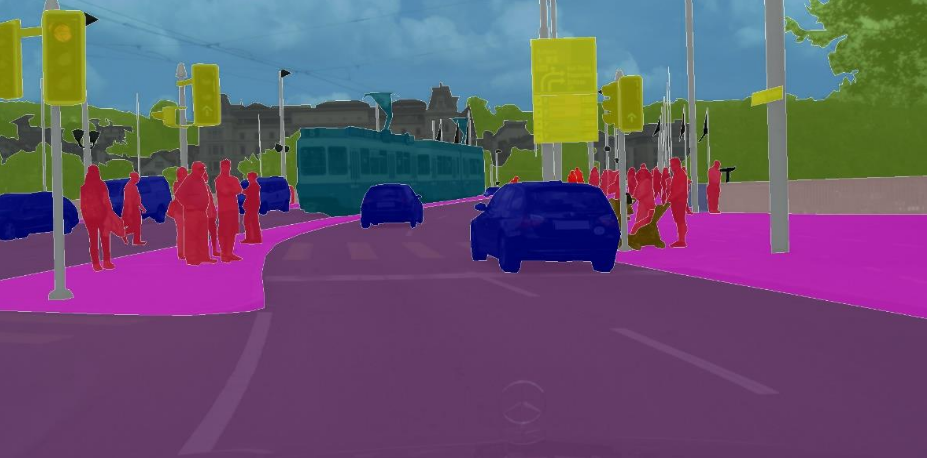
\includegraphics[width=0.7\textwidth]{sections/SemanticSegmentation/img/example.png}

\begin{multicols}{2}
    \subsection{(Non-semantic) Segmentation}
    \begin{itemize}
        \item Find regions in images
        \item No classes or similar information given
        \item Similar to unsupervised learning
        \item Often \glqq bottom-up\grqq{} approach
        \item Compact representation of a scene in terms of regions
        \item Regions share common properties
    \end{itemize}

    \subsubsection{K-Means Clustering}
    Hyperparamter: Number of clusters $N$
    \begin{enumerate}
        \item Initialize Cluster Centers (for example randomly)
        \item Calculate which samples belong to which cluster
        \item Calculate mean values of clusters as new cneters
        \item Iterate over steps 2 and 3 until clusters don't change
    \end{enumerate}
    Clusters shapes are spherical

    \subsubsection{Mean Shift Clustering}
    \begin{enumerate}
        \item For all positions $x$ in the image
              \begin{enumerate}
                  \item Calculate mean $m(x)$ in environment $N(x)$: $m(x)=\dfrac{\sum_{x_i \in N(x)} K(x_i-x_i)x_i}{\sum_{x_i \in N(x)} K(x_i-x_i)}$
                  \item Set $x$ to the mean $m(x)$
                  \item Iterate until $x$ does not change
              \end{enumerate}
    \end{enumerate}
    (Example: Gaussian kernel $K(\frac{x-x_i}{h})=\frac{1}{\sqrt{2\pi}}e^{-\frac{(x-x_i)^2}{2h^2}}$.)
    Clusters shape is variable and not determined by the method

    \subsubsection{Attraction Basins}
    Region, from which all trajectories lead to the same mode
    \begin{enumerate}
        \item Calculate features
        \item Often: include spatial properties (pixel location) in features
        \item Initialize mean shift {\color{red}at each pixel}
        \item Perform mean shift until convergence
        \item Merge starting positions that end up near the same peak into a cluster
    \end{enumerate}

    \subsubsection{Segmentation by Graph Cuts}
    Images as graph:
    \begin{itemize}
        \item Node for every pixel
        \item Edges between Nodes/Pixels (every pair of pixels, neighboring pixels etc.)
        \item Affinity weight for each edge
        \item Measures similarity, for example inversely proportional to difference in color and position
    \end{itemize}
    Graph Cuts
    \begin{itemize}
        \item Let $G = (V,E)$ be a graph.
              Each edge $(u,v)$ has a weight $w(u,v)$ that represents the similarity between $u$ and $v$.
        \item Cut $G$ into 2 disjoint graphs, with node sets $A$ and $B$, by removing all edges between sets $A$ and $B$
        \item Assign a value to the cut as $\text{cut}(A,B) = \sum_{u \in A, v \in B} w(u,v)$
    \end{itemize}
    \paragraph{Min-Cut}
    Of all possible cuts $\text{cut}(A,B)$ select the one with the minimal value
    \paragraph{Normalized Cuts}
    $\text{Ncut}(A,B) = \dfrac{\text{cut}(A,B)}{\text{assoc}(A,V)} + \dfrac{\text{cut}(A,B)}{\text{assoc}(B,V)}$, where $\text{assoc}(A,V) = \sum_{u \in A, t \in V} w(u,t)$ and $V$ is the set of all vertices

    \subsubsection{Superpixels}
    \begin{enumerate}
        \item Calculate superpixels first by grouping similar pixels
        \item Apply normalized graph cuts
    \end{enumerate}
\end{multicols}

\begin{multicols}{2}
    \subsection{Features}
    Features calculate properties of an image or an image region.
    Features should be invariant to:
    \begin{itemize}
        \item Translation
        \item Rotation
        \item Scaling
        \item Illumination changes
    \end{itemize}

    \subsubsection{Local Binary Pattern}
    \begin{itemize}
        \item Analyze the $3\times 3$ neighborhood of a pixel and assign a binary code by comparing the center pixel to the neighbors
        \item Code converted to integer is used as descriptor
    \end{itemize}

    \subsubsection{Filter Banks}
    \begin{itemize}
        \item \textbf{RFS Filters:} Edge and line filters at 6 orientations and 3 scales, Gaussian and Laplacian of Gaussian
        \item \textbf{MR8 Filters:} Maxima of RFS Filters at each scale
    \end{itemize}

    \subsubsection{Textons}
    \begin{itemize}
        \item Texture descriptor as vector of filter bank outputs
        \item Textons found by clustering, called dictionary generation
        \item Similarity between regions by comparison of texton histograms
    \end{itemize}

    \subsubsection{Gray Level Co-Occurence Matrices (GLMCMs)}
    \begin{itemize}
        \item How often a specific combination of a color value between a pixel and its neighbors occur
        \item Results in $256\times 256$ matrix (for 256 gray values)
        \item Additional features can be calculated from the matrix (entropy, energy, homogeneity, contrast, dissimiliarity)
    \end{itemize}

    \subsubsection{Scale Invariant Feature Transform (SIFT)}
    \begin{itemize}
        \item Popular feature descriptor for various tasks such as object matching, image stitching etc.
        \item Combination of detector + descriptor
        \item Descriptor uses histogram of gradient
        \item Results in a 128 dimensional vector
    \end{itemize}

    \subsubsection{Histogram of Oriented Gradients (HoG)}
    \begin{enumerate}
        \item Compute gradient images in $x$ and $y$
        \item Divide image into cells
        \item Compute histogram of gradient orientation (muliplied by gradient value) in cell
        \item Normalize
        \item Flatten into feature vector
    \end{enumerate}

    \subsubsection{HoGgles}
    \glqq Invert\grqq{} HoG features to simulate image that generates it.
    Helps to understand bad detections.

    \subsubsection{Problems with Features \& Classification}
    \begin{itemize}
        \item Many features are available
        \item Not all features work well in all applications
        \item Can be time consumt to find a good feature set and its optimal parameters $\Rightarrow$ Learn features with neural networks
    \end{itemize}
\end{multicols}

\subsection{Metrics}
\begin{tabular}{l l l l}
    Precision = $\frac{t_p}{t_p+f_p}$ & Recall = $\frac{t_p}{t_p+f_n}$  & Specificity = $\frac{t_n}{t_n+f_p}$ & Accuracy = $\frac{t_p+t_n}{t_p+t_n+f_p+f_n}$ \\
    F1 = $\frac{2t_p}{2t_p+f_p+f_n}$  & IoU = $\frac{t_p}{t_p+f_p+f_n}$
\end{tabular}

\subsection{Convolutional Networks}
In order to get a sufficiently large receptive field we need to make very deep networks with large convolutional filters $\Rightarrow$ Use downsampling and upsampling

\subsubsection{Pooling (Downsampling)}
\begin{description}
    \item[Max Pooling:] Take the maximum of a neighborhood and use it as a pixel value in the (smaller) output
    \item[Average Pooling] Take the average of a neighborhood and use it as a pixel value in the (smaller) output
\end{description}

\subsubsection{Unpooling (Upsampling)}
\begin{description}
    \item[Nearest Neighbor:] Reuse the same value in a neighborhood of the output
    \item[Bed of Nails:] Reuse the same value in the upper left corner of the neighborhood and fill the rest with zeros
    \item[Max Unpooling:] Remember the position of the maximum when max pooling and put the value at the correct position in the output. Fill the other values with zeros.
\end{description}

\subsubsection{Convolution}
\begin{description}
    \item[Strided Convolution:] Filter moves $N$ positions in input for every position in output
    \item[Strided Transposed Convolution:] Filter moves $N$ positions in output for every position in input. Summation of values where filter outputs overlap
\end{description}

\subsubsection{Errors}
\begin{description}
    \item[Training Error:] Error on training set
    \item[Generalization Error:] Gap between error on the training and test set
\end{description}

\subsubsection{Regularization}
Limits the capacity of networs by adding a parameter norm penalty to the loss $\tilde{J}(\Theta; X, y) = J(\Theta; X, y) + \alpha \Omega(\Theta)$
\begin{tabular}{l l l l}
    \hline
    Name  & $\Omega(\Theta)$                                        & $\tilde{J}(\Theta; X, y)$                 & $\nabla_w\tilde{J}(\Theta; X, y)$                      \\\hline
    $L^1$ & $\frac{1}{2}\lVert w \rVert^2_1=\sum_i\lvert w_i\rvert$ & $\alpha \lVert w\rVert + J(\Theta; X, y)$ & $\alpha\cdot\text{sign}(w) + \nabla_w J(\Theta; X, y)$ \\
    $L^2$ & $\frac{1}{2}\lVert w \rVert^2_2$                        & $\frac{\alpha}{2}w^T w + J(\Theta; X, y)$ & $\alpha w + \nabla_w J(\Theta; X, y)$                  \\\hline
\end{tabular}
\begin{description}
    \item[Ensemble Methods:] Use several models that are trained separately and then vote on the result
    \item[Drouput:] Randomly drop a node on a hidden layer or an input value. Training learns all sub networks of the original network
    \item[Early Stopping:] Stop when error on validation set starts to increase again. Effectively learn the number of training steps needed.
\end{description}

\subsubsection{Optimization}
Learning is not optimization!
We are interested in a performance measure (on the test set), but we optimize a loss function (on the training set)

\paragraph{Batching}
\begin{itemize}
    \item Used properties in optimization (for example the gradient) are expectations over the training set
    \item Calculating the expectations over the whole data set is very time consuming
    \item We can also calculate them by randomly sampling from the dataset $\rightarrow$ Minibatch algorithms
\end{itemize}
What minibatch size to use?
\begin{itemize}
    \item Large batches $\rightarrow$ better estimates, but with non-linearly increased cost
    \item Very small batches underutilize hardware
    \item Memory might limit batch size in parallel processing
    \item Small batch sizes can offer a regularization effect
\end{itemize}
\textbf{Batch normalization}

\begin{minipage}{0.525\textwidth}
    \begin{itemize}
        \item Usually inserted after convolutional and dense layers before the activation function
        \item Improves gradient flow
        \item Allows higher learning rates
        \item Reduces dependence on (correct) initialization
    \end{itemize}
\end{minipage}
\begin{minipage}{0.475\textwidth}
    \begin{enumerate}
        \item $\mu_B \leftarrow \frac{1}{m}\sum_{i=1}^m x_i$ // mini-batch mean
        \item $\sigma_B \leftarrow \frac{1}{m}\sum_{i=1}^m (x_i-\mu_B)^2$ // mini-batch variance
        \item $\hat{x} \leftarrow \frac{x_i - \mu_B}{\sqrt{\sigma_B^2+\epsilon}}$ // normalize
        \item $y_i \leftarrow \gamma x_i + \beta$ // scale and shift
    \end{enumerate}
\end{minipage}

\paragraph{Stochastic Gradient Descent}
\begin{enumerate}
    \item While not stopping do
          \begin{enumerate}
              \item Sample minibatch of $m$ examples $x^i$, $y^i$
              \item Compute gradient estimate: $\tilde{g}\leftarrow \frac{1}{m}\nabla_\theta \sum_i L(f(x^{(i)};\theta),y^{(i)})$
              \item Apply update: $\theta \leftarrow \theta + \epsilon \tilde{g}$
          \end{enumerate}
\end{enumerate}
Commonly the learning rate is decayed over time $\epsilon_k = (1-\alpha)\epsilon_0 + \alpha \epsilon_\tau$

\paragraph{Momentum}
Accumulate average of past gradients
$v \leftarrow \alpha v - \epsilon \nabla_\theta \left(\frac{1}{m}\sum_i L(f(x^{(i)};\theta),y^{(i)})\right)$, $\theta \leftarrow \theta + v$

\paragraph{Adaptive Learning Rates}
\begin{description}
    \item[Adagrad:] Scales individual learning rates inversely by squared historic gradient. Greater progress for directions with small gradients
    \item[RMSProp:] Similar, but gradient accumulation is done by exponentially weighted moving average
    \item[Adam:] Combination of RMSProp with momentum
\end{description}

\subsubsection{Activation Functions}
\begin{tabular}{l l m{1cm} l l m{1cm} l l}
    Sigmoid & $f(x)=\frac{1}{1+e^-x}$ &  & Softmax    & $f(x)=\frac{e^{x_i}}{\sum_j e^{x_j}}$            & Softplus & $\quad f(x)=\log(1+e^x)$ \\
    ReLU    & $f(x)\max(0,x)$         &  & Leaky ReLU & $f(x)=\left\{\begin{matrix} x, & \text{if } x\geq 0 \\ \alpha x, & \text{if } x<0 \end{matrix} \right.$
\end{tabular}

\begin{multicols}{2}
    \subsubsection{Weight Initialization}
    \begin{itemize}
        \item Too small: Activation go to zero and no learning
        \item Too large: Actiavtion might saturate and no learning
        \item Just right: Nice activation in all layers
    \end{itemize}

    \subsubsection{Learning Process}
    \begin{itemize}
        \item Start with simple/little data and see that your model converges (overfit)
        \item Check loss before and after regularization, check percentage of loss due to regularization
        \item Experiment with learning rate
    \end{itemize}

    \paragraph{Hyperparameter Tuning}
    \begin{itemize}
        \item First coarse search of parameters, then finer search
        \item Most important hyperparameters to try out: Network capacity/architecture, learning rate, decay rate, regularization weights, drouput percentage
    \end{itemize}
\end{multicols}

\subsection{Patches}
\begin{minipage}{0.5\textwidth}
    Idea: Split large images into smaller regions, so called \glqq Patches\grqq.
    \begin{itemize}
        \item Retaining same image size (except border) works well
        \item Little or no max pooling layers perform better
        \item Deeper but \glqq narrower\grqq{} networs perform better
        \item Moderate L2 regularization and dropout improves results
        \item No batch normalization was needed here (but might improve speed of convergence)
        \item Weights on loss functions to correct for unbalanced data sets
    \end{itemize}
\end{minipage}
\begin{minipage}{0.49\textwidth}
    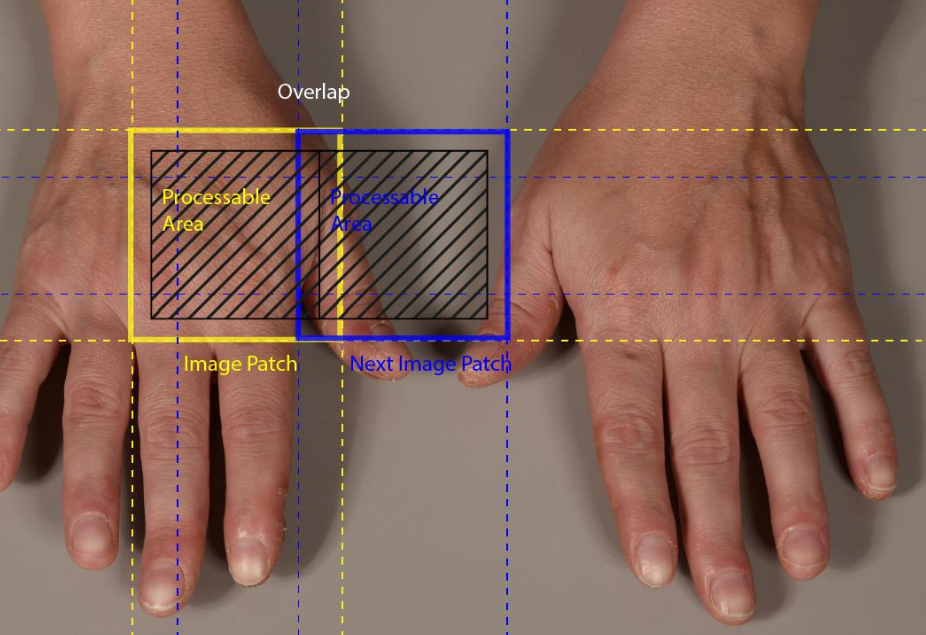
\includegraphics[width=1.0\textwidth]{sections/SemanticSegmentation/img/patches.png}
\end{minipage}
